\chapter{Appendix - Utveckling av webbsida}
\label{app:B}
I appendix B beskrivs först förbättringspunkter angivet från användarna av YATA under iterationscykel 1. Sedan beskrivs en sammanställning av vår användarstudie av Piazza samt en KJ-analys av denna studie. Tillsist presenteras en lista av koncept som stod till grund för valet till MVP A. 

\section{Förbättringspunkter efter iterationscykel 1}
\label{app:itt}

Efter att YATA hade testats för en begränsad mängd studenter med tentamensuppgifter bad vi om återkoppling från dessa studenter på förbättringspunkter på webbplattformen. Följande förbättringspunkter presenterades:

%Från återkopplingen med användarna var detta följande förbätringspunkter från användarna:
\begin{itemize}
    \item Större inmatningsfält.
    \item Mobilanpassad hemsida. 
    \item Uppgifter och kapitel borde inte ändra ordning. 
    \item Det skall alltid exemplifieras vilken form svaret skall matas in på. 
    \item En förvisning som visar om det inmatade svaret har tolkats korrekt. 
    \item I dagsläget syns det inte om sidan registrerat svaret om användaren har fel två gånger i rad. 
    \item Lägg till en buffer för när röda krysset kommer upp, exempelvis en kort animation av krysset.
    \item Svar borde stå kvar i samma ruta då man återkommer till en uppgift, även om uppgiften är löst eller inte. 
\end{itemize}

\newpage

\section{Användarstudie av Piazza}
\label{app:surveypiazza}
Nedan presenteras dokumentet som användes för användarstudien av Piazza. 

\begin{figure}[H]
    \centering
    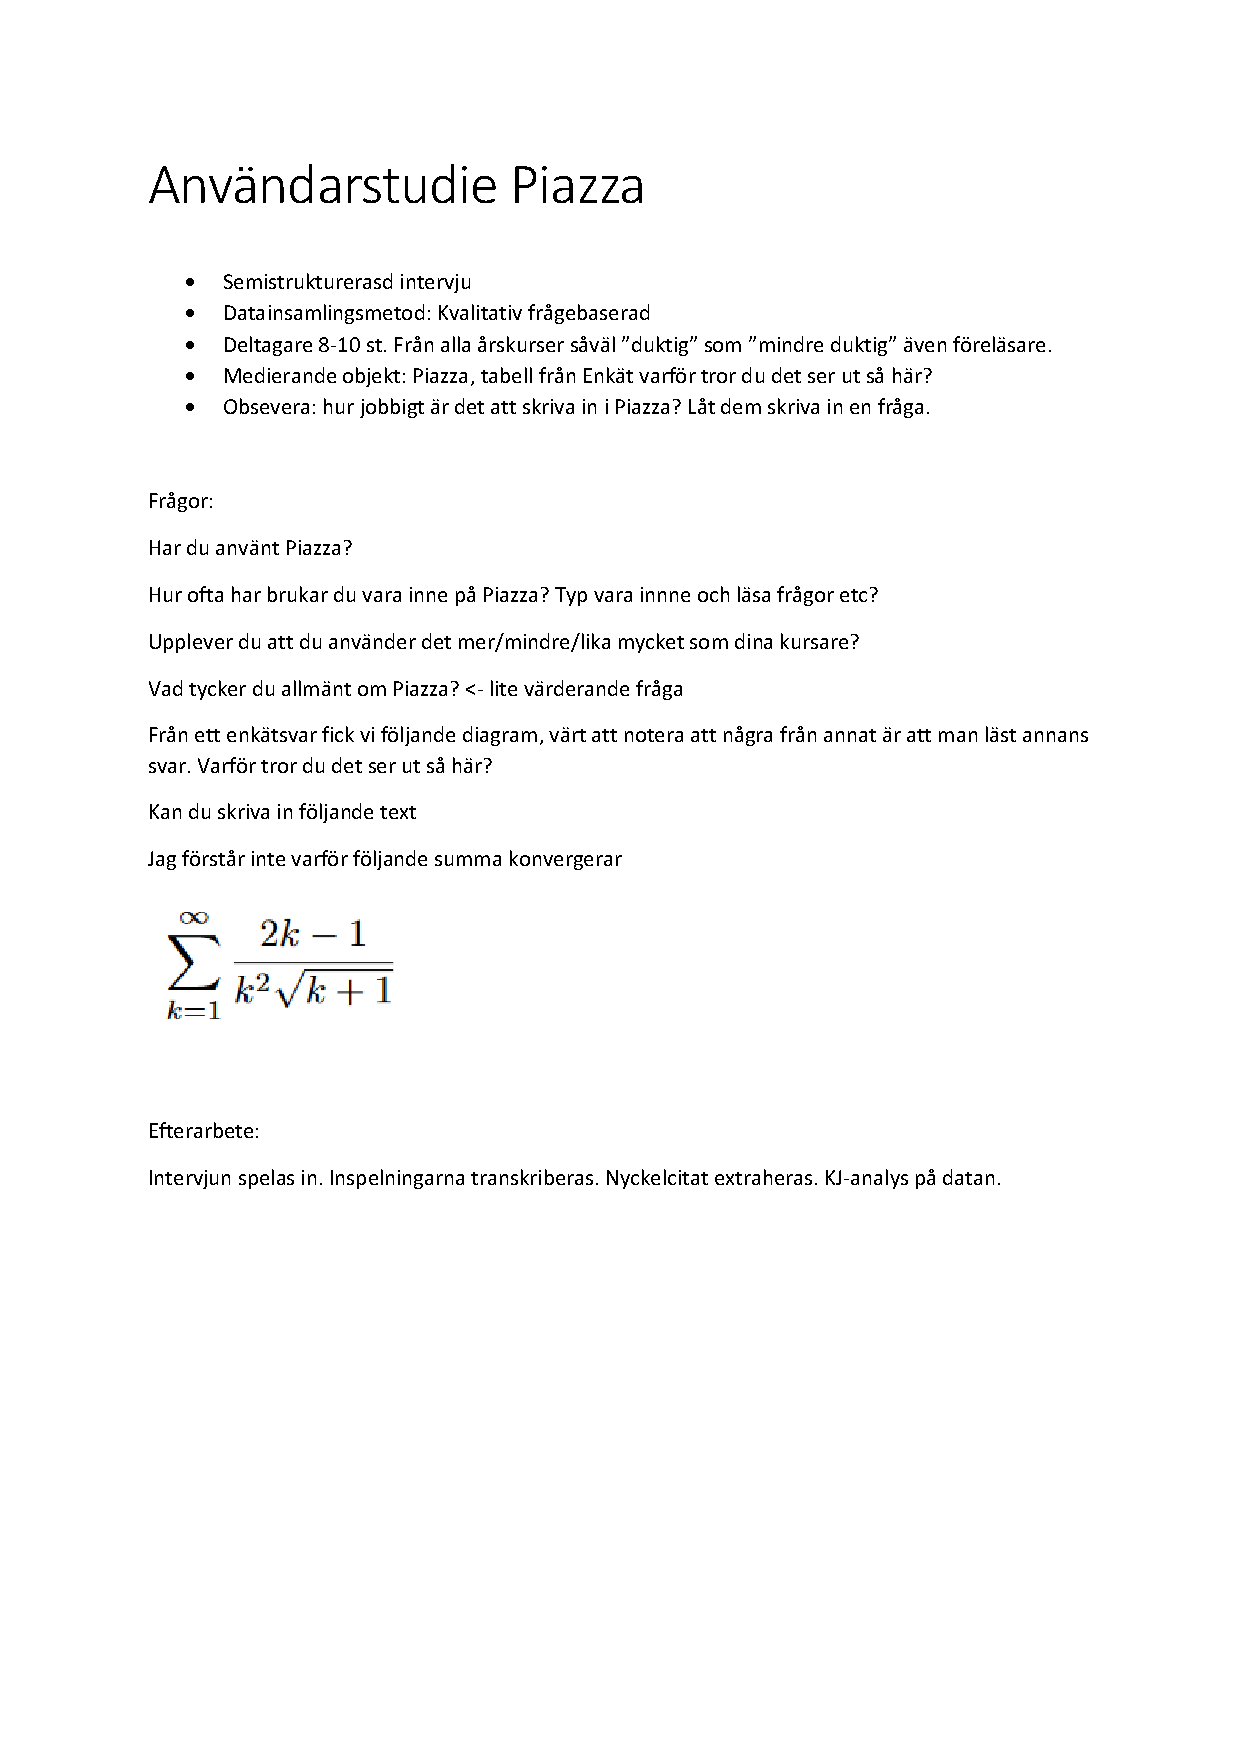
\includegraphics[scale=0.75]{appendix/userstudy_piazza.pdf}
    \caption*{Sammanställning av användarstudie (Piazza)}
    \label{fig:piazzausersurvey}
\end{figure}

\section{KJ-analys av Piazza}
\label{app:KJ-analys}
KJ-analys bygger på att samla flera människors perspektiv av samma information för att tillmammans få en bättre bild av det analyserade materialet \cite{kj}. Det specifika fallet av arbetes KJ-analys av Piazza analyserades studenters användning av Piazza i from av transkriberade intervjuer. Den transkriberade texten delades in i enskilda kommentarer där varje kommentar analyserades av samtliga medlemmar och kategoriserades sedan enligt vad majoriteten av gruppen tyckte var lämpligt. Nedan presenteras resultatet av KJ-analysen i from av en illustration gjord i programmet Figma \cite{figma}. På grund av storleken av illustrationen har den roterats och delats upp i flera delar.

\begin{figure}[H]
    \centering
    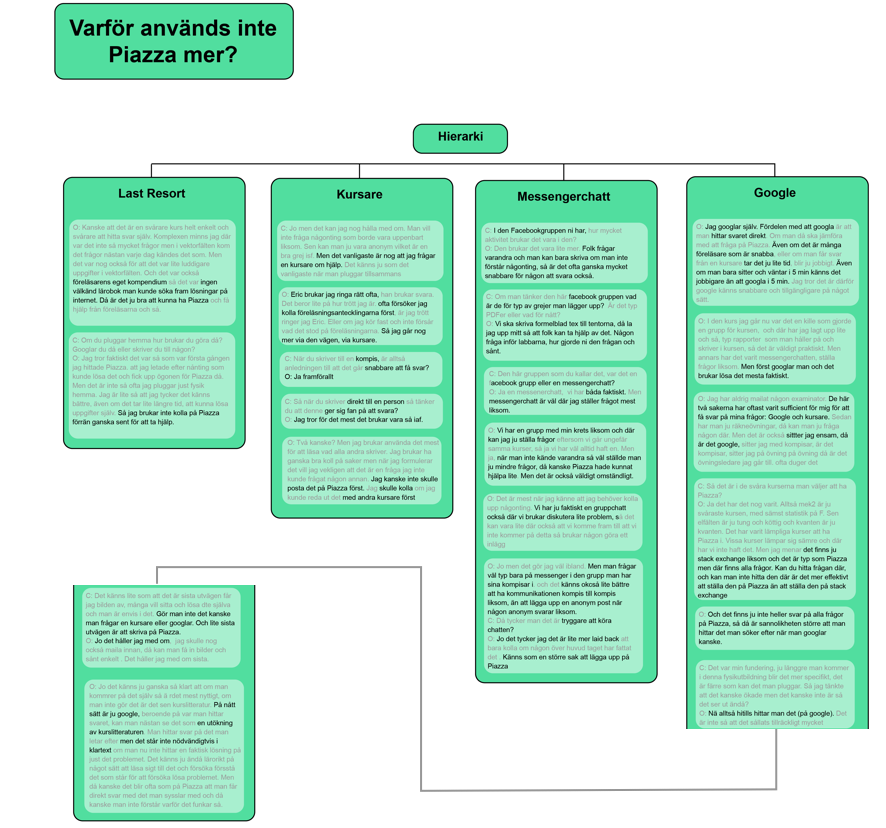
\includegraphics[scale=0.65,angle=90]{appendix/appendix_green/part3.png}
    \caption*{}
    \label{fig:nr8_part4}
\end{figure}

\begin{figure}[H]
    \centering
    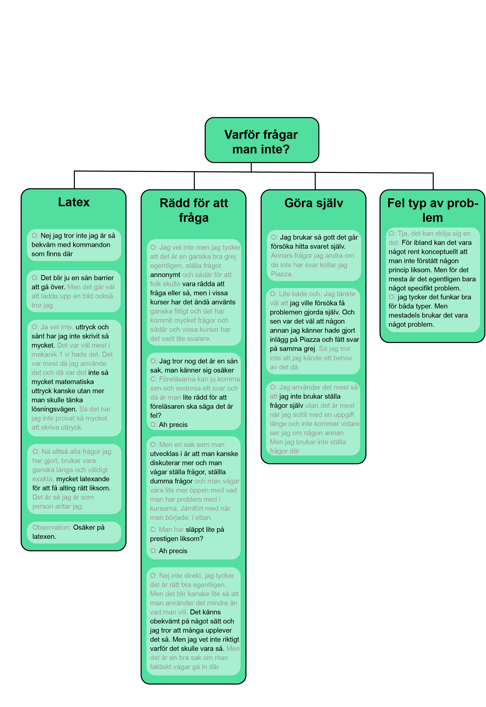
\includegraphics[scale=0.75,angle=0]{appendix/appendix_green/part1.png}
    \caption*{}
    \label{fig:nr8_part10}
\end{figure}

\begin{figure}[H]
    \centering
    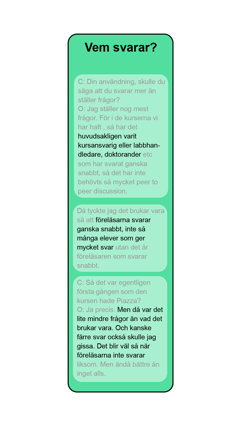
\includegraphics[scale=0.75,angle=90]{appendix/appendix_green/part2.png}
    \caption*{}
    \label{fig:nr8_part5}
\end{figure}

\begin{figure}[H]
    \centering
    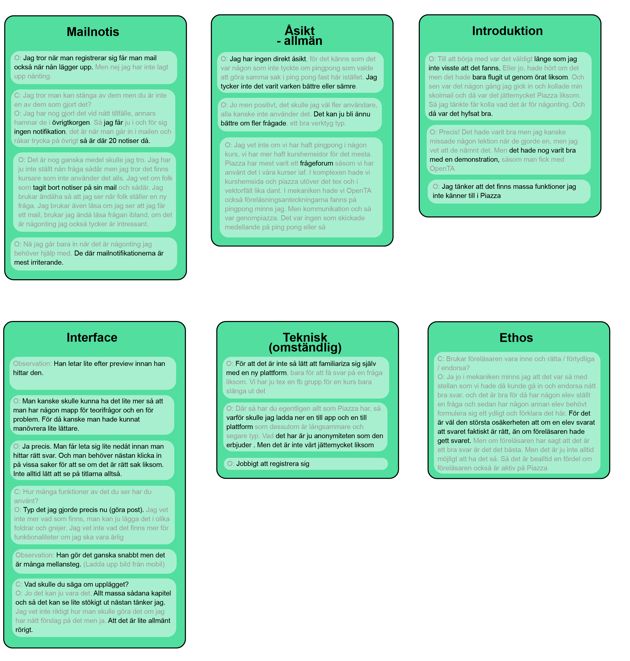
\includegraphics[scale=0.75,angle=90]{appendix/appendix_green/part4.png}
    \caption*{}
    \label{fig:nr8_part6}
\end{figure}

\begin{figure}[H]
    \centering
    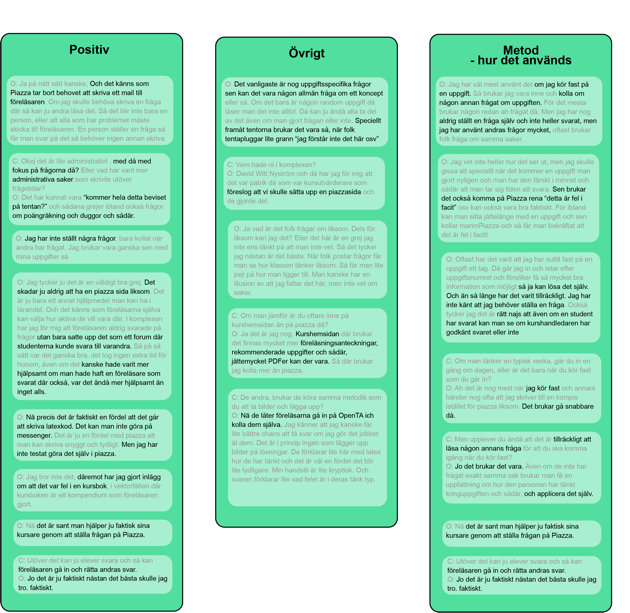
\includegraphics[scale=0.8,angle=90]{appendix/appendix_green/part5.png}
    \caption*{}
    \label{fig:nr8_part7}
\end{figure}

\begin{figure}[H]
    \centering
    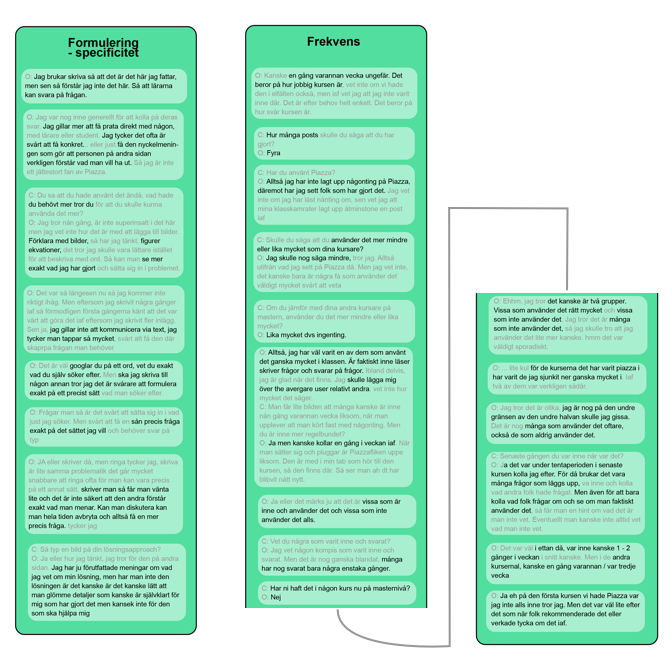
\includegraphics[scale=0.8,angle=90]{appendix/appendix_green/part6.png}
    \caption*{}
    \label{fig:nr8_part8}
\end{figure}

\newpage

\section{Lista av koncept till MVP A}
\label{app:koncept}

I följande lista visar vi de koncept på MVP A vi kom på under en idégenerering med fokus på problematiken att många kör fast i lösningsgångar. Notera att det var punkt nr 5 som vi slutligen bestämde oss för att utveckla:
\begin{itemize}
    \item Användaren tar kort på sin lösningsgång och laddar upp den på webbsidan. Detta kan sedan användas som fullständigt lösningsförslag åt andra studenter. Bilden  skulle också kunna användas som tips genom att användaren exempelvis successivt får se 25 procent av bilden i flera steg. 
    \item En chattfunktion som sammankopplar studenterna. Exempelvis skulle man kunna koppla samman en student som löst en uppgift med en som kört fast på samma uppgift. Alternativt skulle man kunna koppla ihop studenter som är på samma uppgift men ännu inte löst den för att diskutera hur de tänker.  
    \item Ett kommentarsfält under varje uppgift, exempelvis som Youtube har ett kommentarsfält under varje video.   
    \item En AI chattbot som studenten kan ställa frågor till och få svar. 
    \item En tipsfunktion där en användare som löst en uppgift får möjligheten att skriva in ett tips för hur uppgiften kan lösas. Detta tips kan sedan visas för någon som kört fast på samma uppgift.
    \item En direktlänk till Google från webbsidan. Webbsidan skulle då kunna spara bra länkar som studenter hittar, vilka kan användas av andra senare.  
    \item En mall som studenten går igenom när den kört fast där de svarar på frågor exempelvis: ''Det här förstår jag'', ''Så här långt har jag kommit'', ''Det här är min lösningsansättning'' och ''Vad jag inte förstår är''. Detta skulle kunna hjälpa studenten, men också användas som ett sätt för andra att felsöka dess lösning, liknande som Githubs sätt att rapportera buggar.  
\end{itemize}